\thispagestyle{plain}
\chapter{Diseño y Desarrollo del Prototipo}
	\section{Prototipo del Circuito del Termómetro}
		\par
			El prototipo del circuito del termómetro consta de tres versiones: un termómetro  sin capacidades de comunicación inalambrica el cual llamaremos "sencillo", un termómetro con capacidades inalambricas RF 2.4 GHz el cual llamaremos "nodo" y un termómetro con capacidades inalambricas RF 2.4 GHz y bluetooth 2.0 el llamaremos "madre".
			
		\subsection{Circuito ``Sencillo"}
	\par 
		El circuito del termómetro sencillo es la base de la sección de electronica en este proyecto. Un termómetro esencialmente es sensor el cual una de sus caracteristicas fisicas es susceptible a los cambios de temperatura y un indicador de temperatura que muestra en una escala de temperatura que nosotros los seres humanos interpretamos.
		
	\par
		El sensor utilizado es el DS18B20, debido a sus caracteristicas y bajo precio, el sensor solamente necesita una fuente de poder de 5V para trabajar. El Arduino trabajara como interprete de los valores del sensor, basicamente trabaja como un puente entre el sensor de temperatura y el indicador de temperatura. Como podemos ver en la figura 4.1 el DS18B20 se comunica con el arduino a travez de una resistencia de 4.7K ohms, esto permite al arduino captar los valores del sensor utilizando solamente un pin digital. 
		
\clearpage
\thispagestyle{plain}

	\begin{figure}[H]
		\centering
		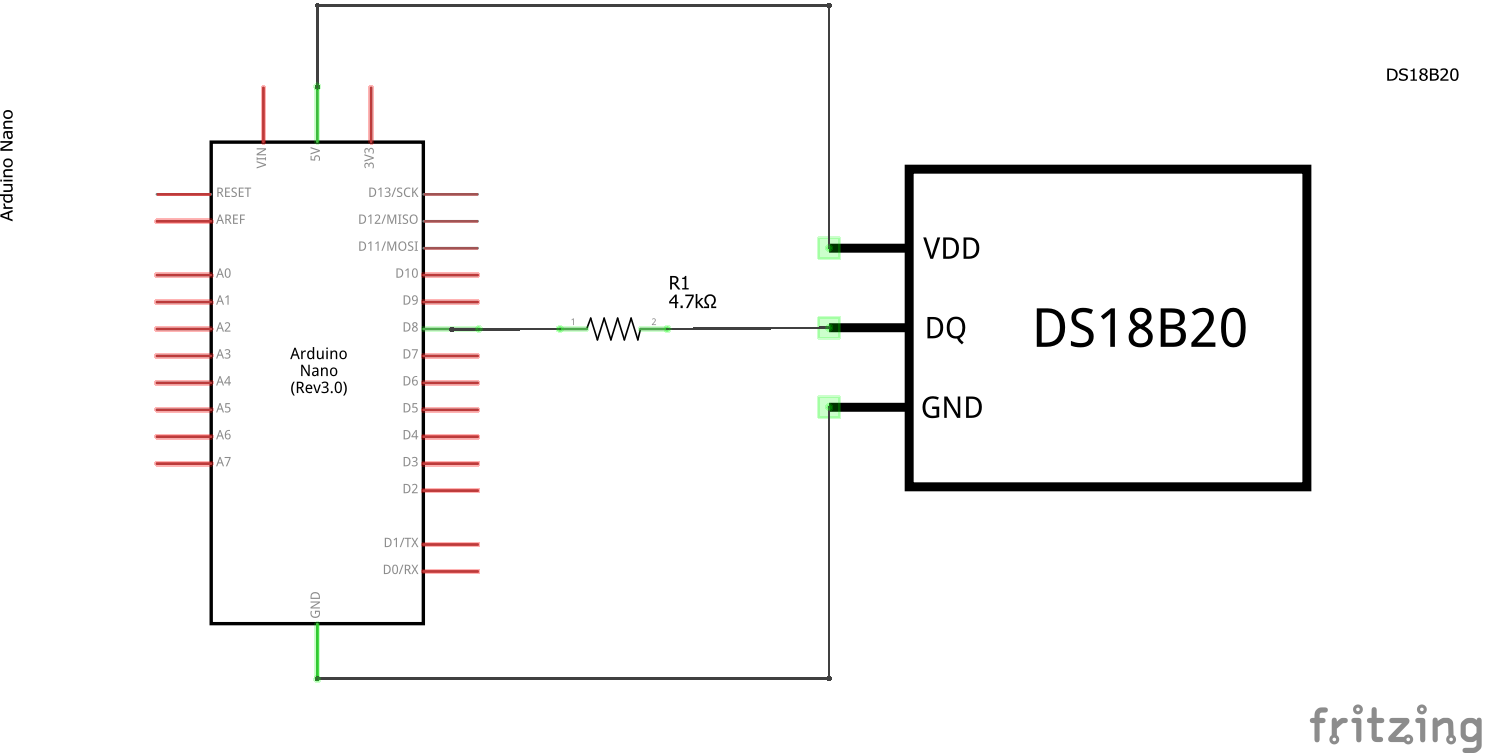
\includegraphics[width=12cm, height=6cm]{sencillo1_schematic.png}
		\caption{Esquemático de conexión del sensor DS18B20 al arduino}
	\end{figure}

	\par 
		La pantalla LCD que utilizaremos es el Nokia 5110, debido a que permite una comunicación sencilla con nuestro arduino la unica limitante es 
		
		\subsection{Circuito ``Nodo"}
		
		\subsection{Circuito ``Madre''}

\clearpage
\thispagestyle{plain}
		
		